% =============================================================================
% sections/03_final_design_description.tex  -  Section 3: Final Design Description
% Teams: all / Status: rover side scaffolded, drone side pending
%
% SCORING (0-40 pts):
%   Rover structure (0-6): PT, WBS, OBS - both rover and drone (0-2);
%     rover design description (0-1); rover technical budgets: mass, power,
%     data link (0-1); critical parts for on-site ERC tasks (0-1);
%     innovative design solutions highlighted (0-1)
%   Rover design description excellence (0-20)
%   Drone structure (0-4): description (0-1); budgets: mass, power, data
%     link (0-1); critical parts (0-1); innovations (0-1)
%   Drone excellence (0-10; 0 pts if fully COTS drone)
%
% The drone side is an acknowledged gap: the subsections below exist
% because the rubric requires them, but no leaf files exist yet since their
% content hasn't been discussed.
%
% Ordering lives only here (ai_context/DECISIONS.md) - leaf files under
% sections/design/ have stable, unnumbered names and contain body content
% only, no \subsection/\subsubsection commands of their own.
% =============================================================================

\section{Final Design Description}
\label{sec:design}

\subsection{Product Tree, Work Breakdown Structure, and Organisation Breakdown Structure}
\label{subsec:pt_wbs_obs}

\subsubsection{Product Tree}
\label{subsubsec:product_tree}
% =============================================================================
% sections/design/breakdowns/product_tree.tex  -  Product Tree
% Teams: PM / Status: stub
%
% Page budget: 1 x A4 total, for BOTH rover and drone on one page. If both
% don't fit legibly, split into product_tree_rover.tex /
% product_tree_drone.tex and update the assembler accordingly.
%
% Source: update the Preliminary Report's rover/drone product tree figures
% rather than redrawing from scratch. Diagrams are drawn outside LaTeX and
% imported as exported PDFs (ai_context/DECISIONS.md).
% =============================================================================

\todo[inline]{Product Tree (rover + drone). Update from the Preliminary
Report's product tree figures. Export as PDF into figures/ and include it
here.}


\subsubsection{Work Breakdown Structure}
\label{subsubsec:wbs}
% =============================================================================
% sections/design/breakdowns/wbs.tex  -  Work Breakdown Structure
% Teams: PM / Status: stub
%
% Page budget: 1 x A4. New for the Final Report - did not exist in the
% Preliminary. Work packages, not yet drafted anywhere. Diagram drawn
% outside LaTeX, exported as PDF (ai_context/DECISIONS.md).
% =============================================================================

\todo[inline]{Work Breakdown Structure diagram. New content - no prior
version to update. Export as PDF into figures/ and include it here.}


\subsubsection{Organisation Breakdown Structure}
\label{subsubsec:obs}
% =============================================================================
% sections/design/breakdowns/obs.tex  -  Organisation Breakdown Structure
% Teams: PM / Status: stub (diagram not yet drawn)
%
% =============================================================================

\todo[inline]{Organisation Breakdown Structure diagram (team org chart).
New content - no prior version to update. Draw outside LaTeX and export it
to replace the placeholder at \autoref{fig:obs_diagram}.}


\subsection{Rover Design Description}
\label{subsec:rover_design_description}

\subsubsection[Rover's Design Overview]{Rover's Design Overview\exampleflag}
\label{subsubsec:rover_design_overview}
\input{sections/design/rover/design_overview}

\subsubsection[Robotic Hand Overview]{Robotic Hand Overview\exampleflag}
\label{subsubsec:robotic_hand_overview}
\input{sections/design/rover/robotic_hand_overview}

\subsubsection[Science Container]{Science Container\exampleflag}
\label{subsubsec:science_container}
% =============================================================================
% sections/design/rover/science_container.tex  -  Science Container
% Teams: science (best guess - unconfirmed) / Status: EXAMPLE (scope approximation)
%
% EXAMPLE CONTENT for scope/layout approximation - not final report text.
% Adapted from the Preliminary Report's "Sample Storage and Weighing
% System" subsection, trimmed to minimal prose. Detailed mechanism
% (servo-driven lid, load-cell tilt-compensation formula, CAN transmission)
% deferred to a later/deeper section rather than crammed in here.
% Marked with \exampleflag on its heading in the assembler.
%
% Images are placeholders (teams/science/figures/*.png) - swap them for the
% real scheme/photos by overwriting the same files.
%
% NOTE: this subsection is meant to fully cover the science container; do
% not repeat this content elsewhere in the report.
% =============================================================================

The science container stores collected samples in three independent,
load-cell-monitored cups -- regolith, rock, and deep-sample -- housed in a
\qtyproduct{503 x 180 x 120}{\milli\meter} outer enclosure mounted on the
front chassis, shown in \autoref{fig:science_container_scheme}. Rock
specimens up to \qty{15}{\centi\meter} and the \qty{35}{\milli\meter} auger
diameter are accommodated by dedicated cup geometries. Each cup weighs its
contents to a resolution of $\pm\,$\qty{1}{\gram}, independent of rover
tilt. The container in use is pictured in
\autoref{fig:science_container_action}.

\begin{figure}[!htbp]
    \centering
    \setlength{\fboxsep}{0pt}

    \begin{minipage}[c]{0.49\textwidth}
        \centering
        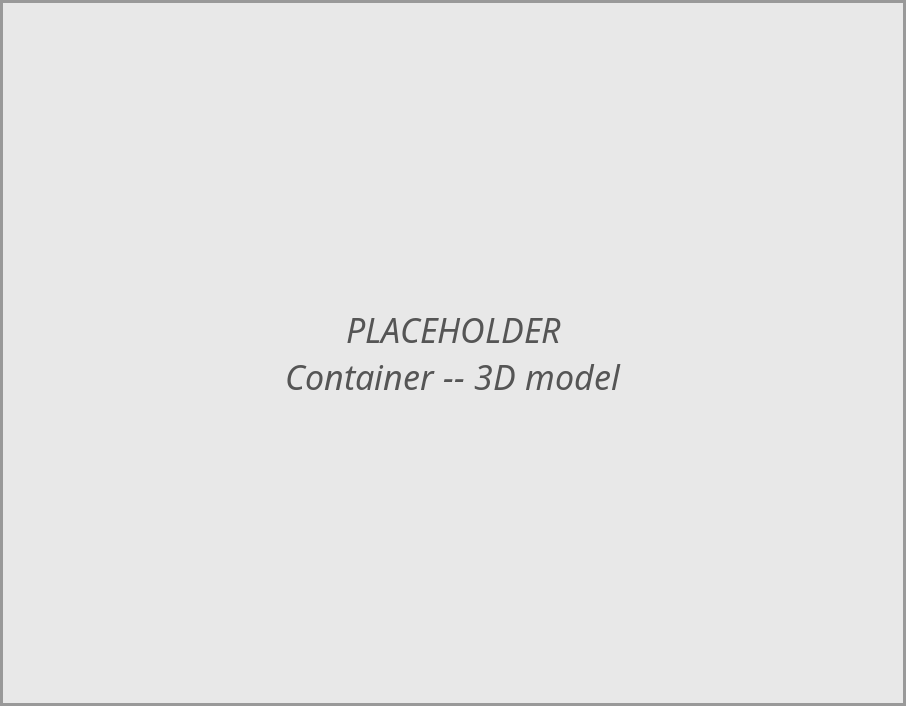
\includegraphics[height=3.5cm, keepaspectratio]{teams/science/figures/container_3d_model}
    \end{minipage}
    \hfill
    \begin{minipage}[c]{0.49\textwidth}
        \centering
        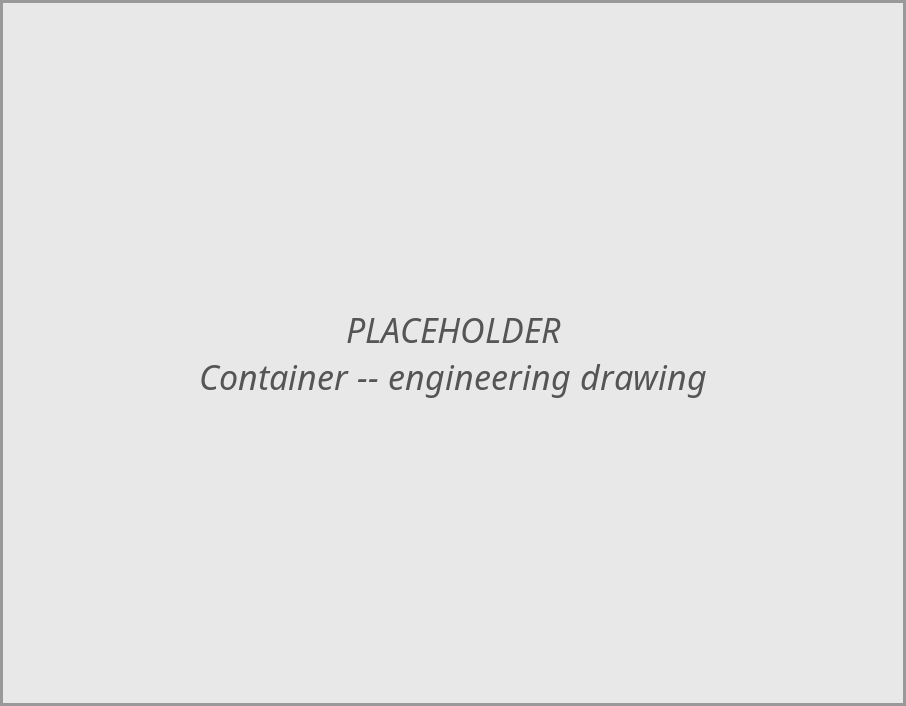
\includegraphics[height=3.5cm, keepaspectratio]{teams/science/figures/container_drawing}
    \end{minipage}

    \caption{Sample storage container: 3D model (left) and engineering drawing (right)}
    \label{fig:science_container_scheme}
\end{figure}

\begin{figure}[!htbp]
    \centering
    \setlength{\fboxsep}{0pt}

    \begin{minipage}[c]{0.49\textwidth}
        \centering
        
\includegraphics[height=3.5cm, keepaspectratio]{teams/science/figures/collecting_sand}
    \end{minipage}
    \hfill
    \begin{minipage}[c]{0.49\textwidth}
        \centering
        
\includegraphics[height=3.5cm, keepaspectratio]{teams/science/figures/collecting_rock}
    \end{minipage}

    \caption{Science container in use: collecting regolith (left) and a rock specimen (right)}
    \label{fig:science_container_action}
\end{figure}


\subsubsection[Electronics Overview]{Electronics Overview\exampleflag}
\label{subsubsec:rover_electronics_overview}
% =============================================================================
% sections/design/rover/electronics_overview.tex  -  Electronics Overview
% Teams: electronics (best guess - unconfirmed) / Status: EXAMPLE (scope approximation)
%
% EXAMPLE CONTENT for scope/layout approximation - not final report text.
% Adapted from the Preliminary Report's "Battery Configuration and
% Hot-Swap Design" / "Power Distribution and Regulation" subsections,
% trimmed to minimal prose. Marked with \exampleflag on its heading in the
% assembler.
%
% Image is a placeholder (teams/electronics/figures/power_distribution_schematic.png)
% - swap it for the real schematic by overwriting the same file.
% =============================================================================

The rover's power system is built around a \qty{48}{\volt} DC bus, with
three to four hot-swappable commercial lithium-ion battery modules
(\qty{48}{\volt}, \qty{12}{\ampere\hour} each) connected in parallel,
giving \qtyrange{36}{48}{\ampere\hour} of capacity depending on mission
demand. Modules mount on a rail-based hot-swap dock for tool-free
replacement in the field and include integrated BMS protection with
current sharing across modules. Power is split into two segments, shown in
\autoref{fig:power_distribution_schematic}: an always-on Safety and
Control Segment, powered directly off the bus ahead of the main
contactor, that regulates \qty{24}{\volt}, \qty{5}{\volt}, and
\qty{3.3}{\volt} rails for the emergency-stop system, control logic, and
communications even with main power disconnected; and a Main Power
Segment, activated via the main contactor, that distributes
\qty{48}{\volt}, \qty{24}{\volt}, \qty{5}{\volt}, and \qty{3.3}{\volt}
rails to all operational consumers.

\begin{figure}[!htbp]
    \centering
    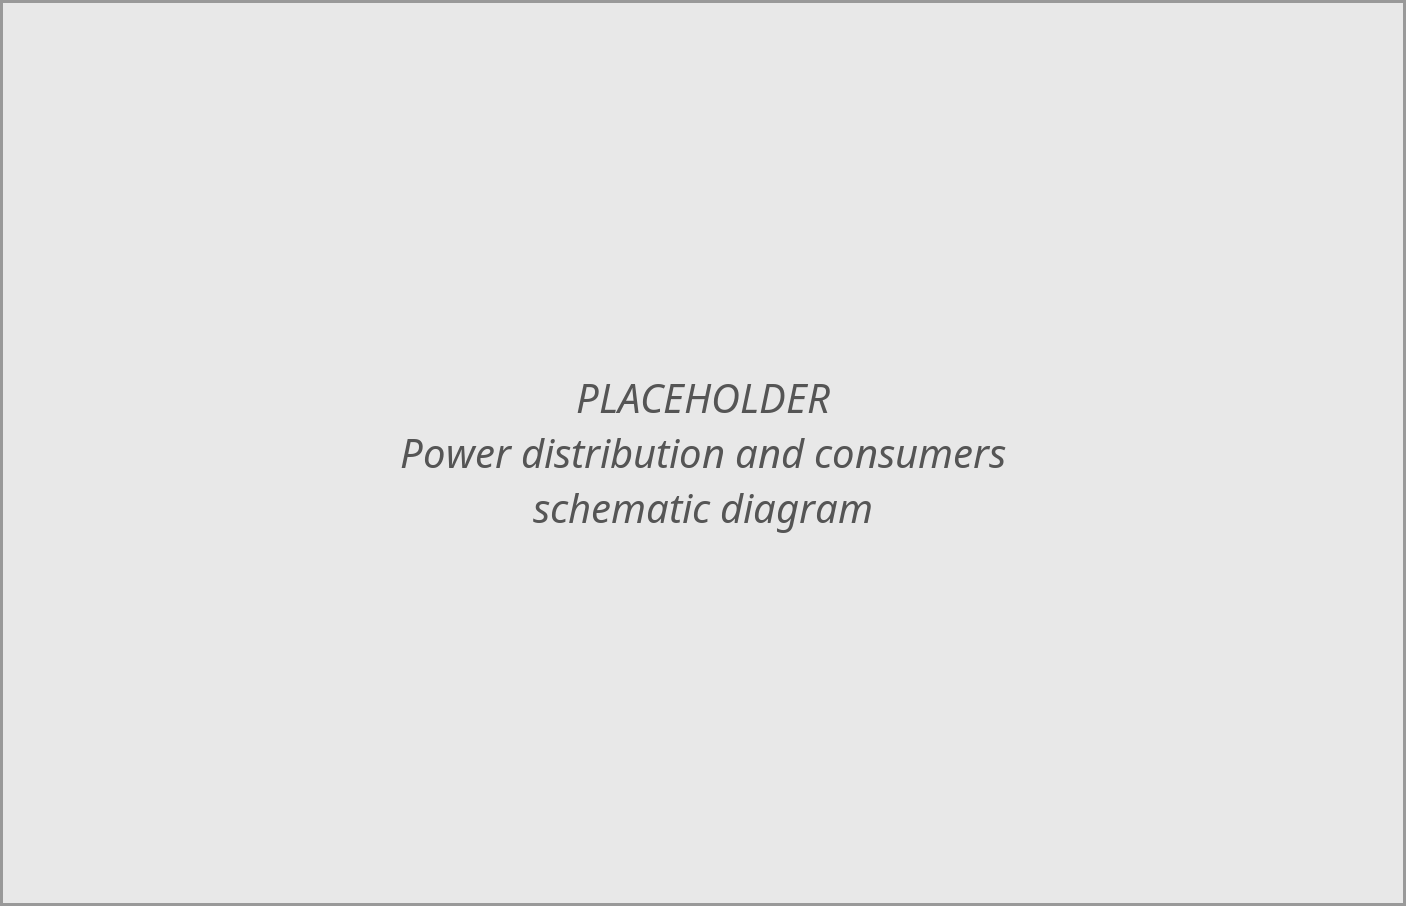
\includegraphics[width=0.85\linewidth]{teams/electronics/figures/power_distribution_schematic}
    \caption{Power distribution and consumers schematic diagram}
    \label{fig:power_distribution_schematic}
\end{figure}


\subsubsection[Ground Station Overview]{Ground Station Overview\exampleflag}
\label{subsubsec:ground_station_overview}
% =============================================================================
% sections/design/rover/ground_station_overview.tex  -  Ground Station Overview
% Teams: ground_station (best guess - unconfirmed) / Status: EXAMPLE (scope approximation)
%
% EXAMPLE CONTENT for scope/layout approximation - not final report text.
% Adapted from the Preliminary Report's "Ground Station Setup and
% Equipment" subsection, trimmed to minimal prose. Marked with \exampleflag
% on its heading in the assembler.
%
% Images are placeholders (teams/ground_station/figures/gs_*.png) - swap
% them for the real scheme/photo by overwriting the same files.
% =============================================================================

The Ground Station Unit (GSU) provides operators with real-time control,
data visualization, and status monitoring. Its core setup includes a
ground station PC for video decoding and telemetry, a user interface with
two monitors, a control panel, and a rover controller for manual
navigation, plus a tripod-mounted directional antenna connected via
Ethernet within a \qty{20}{\meter} radius, shown in
\autoref{fig:ground_station_setup}.

\begin{figure}[!htbp]
    \centering
    \setlength{\fboxsep}{0pt}

    \begin{minipage}[c]{0.49\textwidth}
        \centering
        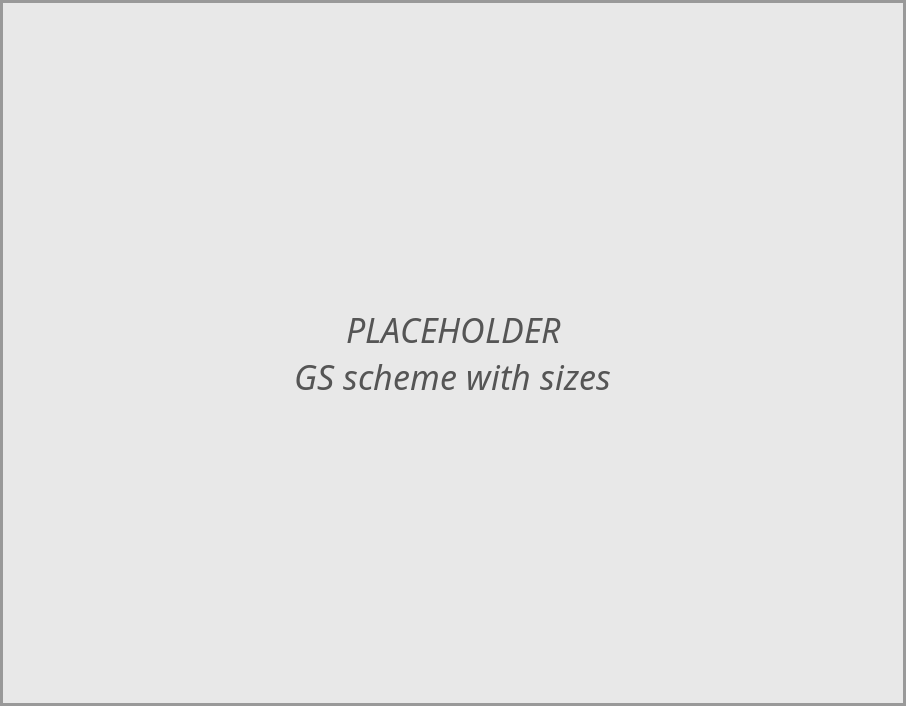
\includegraphics[height=3.5cm, keepaspectratio]{teams/ground_station/figures/gs_scheme}
    \end{minipage}
    \hfill
    \begin{minipage}[c]{0.49\textwidth}
        \centering
        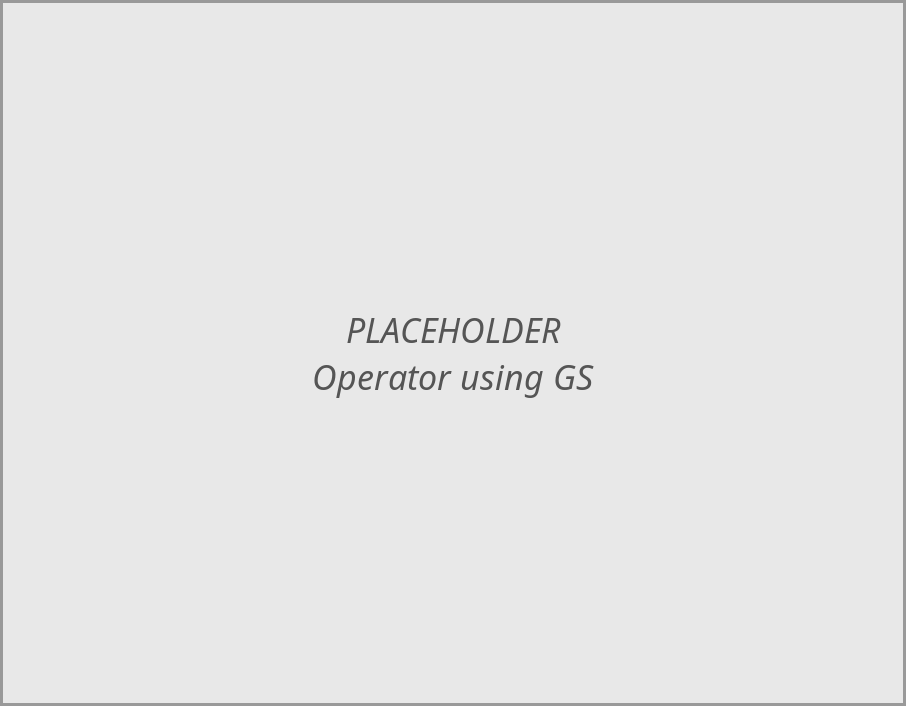
\includegraphics[height=3.5cm, keepaspectratio]{teams/ground_station/figures/gs_operator}
    \end{minipage}

    \caption{Ground Station Unit: scheme with sizes (left) and operator in use (right)}
    \label{fig:ground_station_setup}
\end{figure}


\subsubsection[Hardware Overview]{Hardware Overview\exampleflag}
\label{subsubsec:rover_hardware_overview}
% =============================================================================
% sections/design/rover/hardware_overview.tex  -  Hardware Overview
% Teams: electronics (best guess - unconfirmed) / Status: EXAMPLE (scope approximation)
%
% EXAMPLE CONTENT for scope/layout approximation - not final report text.
% Adapted from the Preliminary Report's "System Architecture Wiring
% Diagram" subsection, trimmed to minimal prose. Marked with \exampleflag
% on its heading in the assembler.
%
% Image is a placeholder (figures/hardware_architecture.png) - swap it for
% the real wiring diagram by overwriting the same file. Shared figures/
% (not a team folder) since this is a whole-rover, system-level diagram.
% =============================================================================

The rover's onboard hardware is organized around a main computer that
performs high-level processing and sensor collection, primarily over USB,
coordinating with subsystem controllers over CAN and Ethernet: a chassis
controller drives the wheels, an arm controller manages actuators, sensors,
and the arm context camera, and dedicated science and operation subsystems
handle sampling instruments and external communication. The resulting
wiring architecture is shown in \autoref{fig:hardware_architecture}.

\begin{figure}[!htbp]
    \centering
    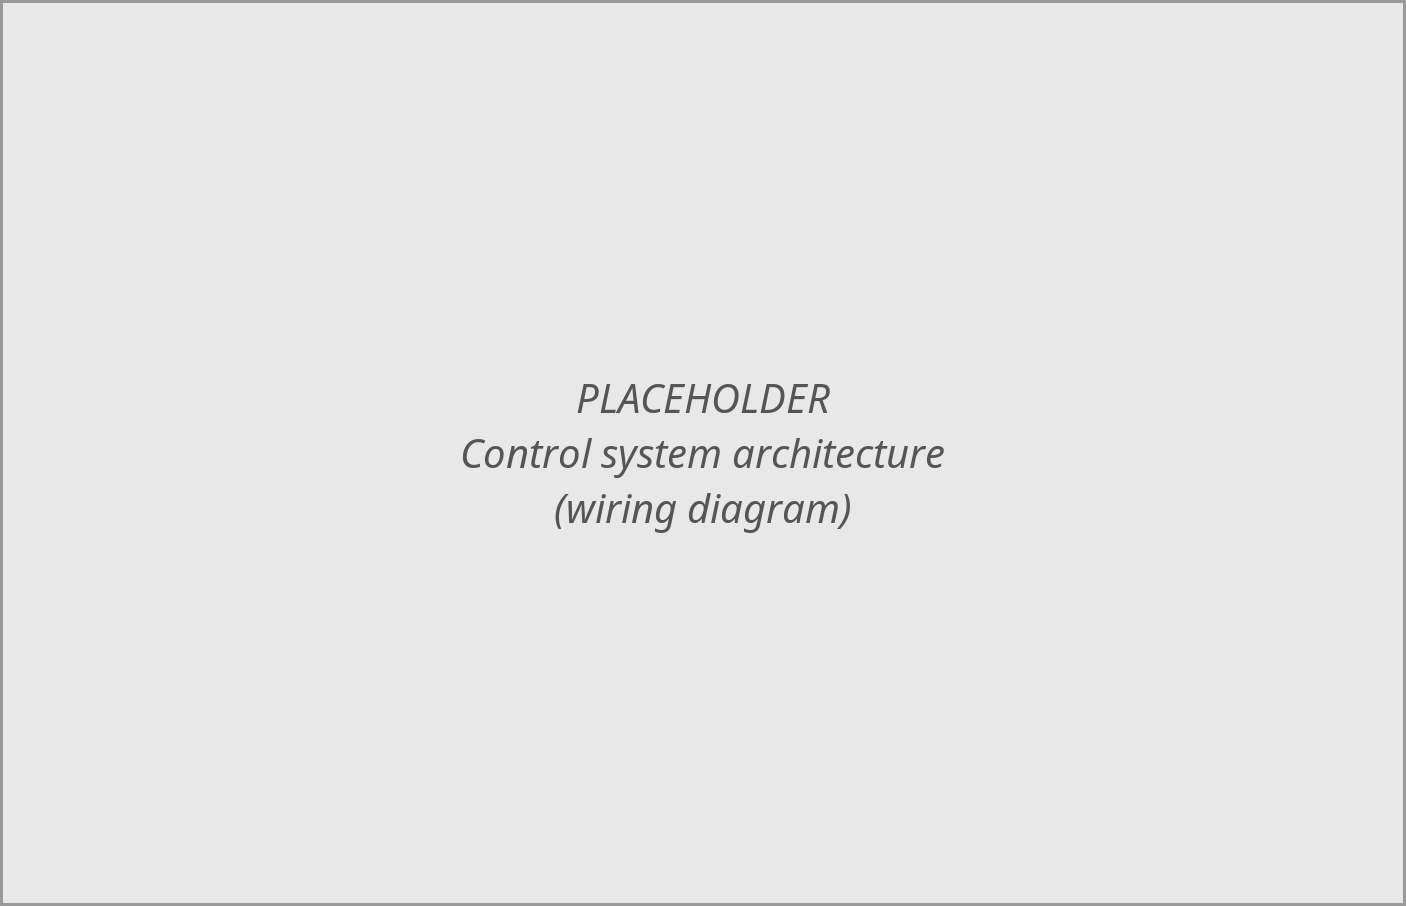
\includegraphics[width=0.85\linewidth]{figures/hardware_architecture}
    \caption{Control system architecture}
    \label{fig:hardware_architecture}
\end{figure}


\subsubsection[Software Overview]{Software Overview\exampleflag}
\label{subsubsec:rover_software_overview}
% =============================================================================
% sections/design/rover/software_overview.tex  -  Software Overview
% Teams: electronics / navigation (best guess - unconfirmed) / Status: EXAMPLE (scope approximation)
%
% EXAMPLE CONTENT for scope/layout approximation - not final report text.
% Adapted from the Preliminary Report's "Software Architecture" intro,
% trimmed to minimal prose. Marked with \exampleflag on its heading in the
% assembler.
%
% Image is a placeholder (figures/software_architecture.png) - swap it for
% the real ROS 2 node graph by overwriting the same file. Shared figures/
% (not a team folder) since this is a whole-rover, system-level diagram.
% =============================================================================

The rover's software stack is built on ROS 2 Humble as the middleware
framework, providing standardized inter-process communication via topics,
services, and actions, and integrating with the broader ROS 2 ecosystem of
navigation, perception, and control packages used throughout the system.
\autoref{fig:software_architecture} shows the resulting node-level
architecture.

\begin{figure}[!htbp]
    \centering
    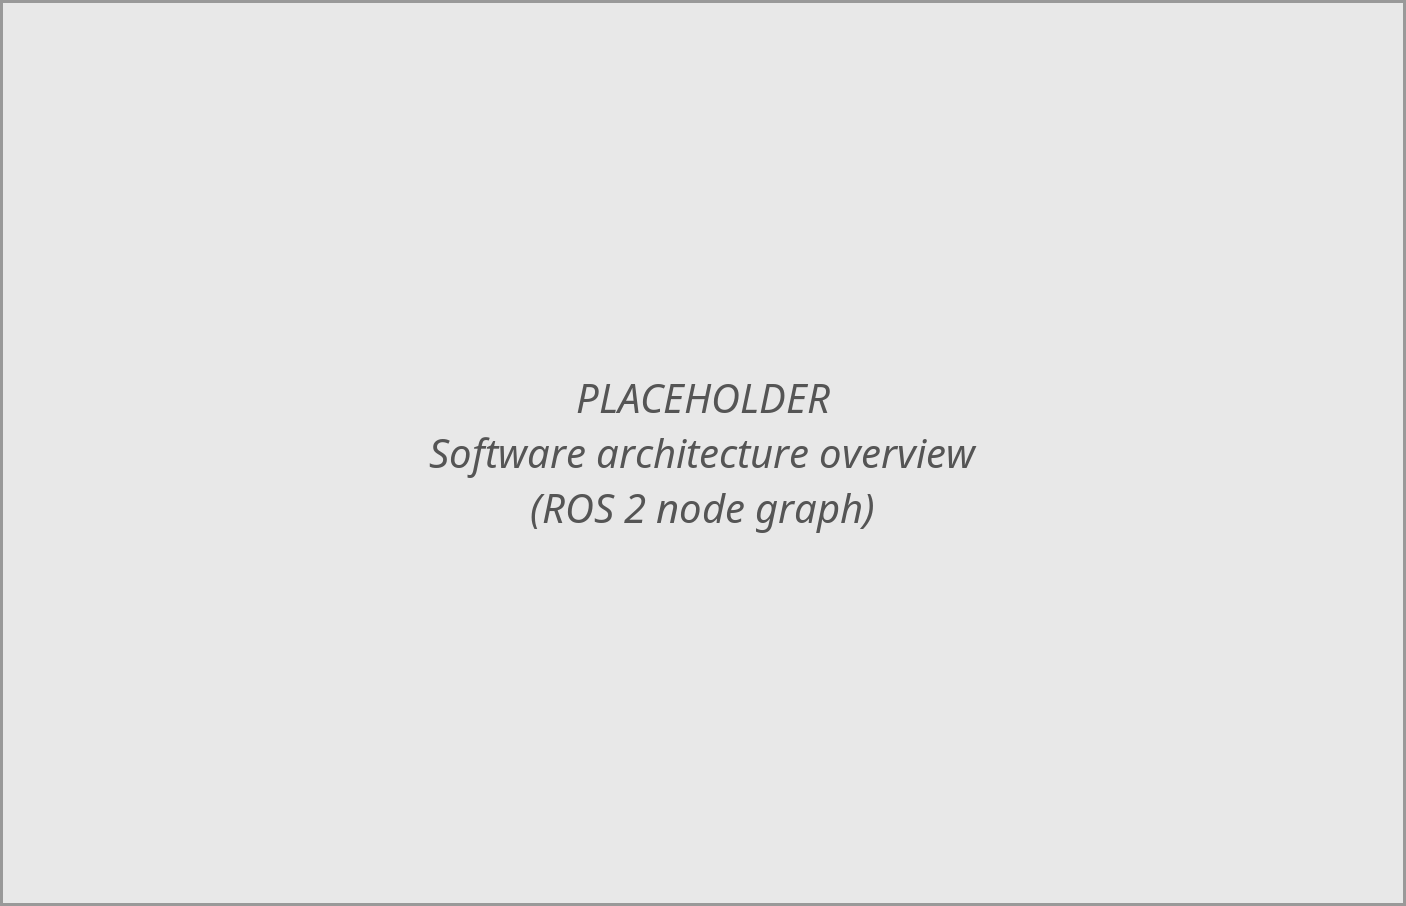
\includegraphics[width=0.85\linewidth]{figures/software_architecture}
    \caption{Software architecture overview}
    \label{fig:software_architecture}
\end{figure}


\subsubsection[Communication Overview]{Communication Overview\exampleflag}
\label{subsubsec:rover_communication_overview}
\input{sections/design/rover/communication_overview}

\subsubsection[Navigational Stack]{Navigational Stack\exampleflag}
\label{subsubsec:navigational_stack}
% =============================================================================
% sections/design/rover/navigational_stack.tex  -  Navigational Stack
% Teams: navigation (best guess - unconfirmed) / Status: EXAMPLE (scope approximation)
%
% EXAMPLE CONTENT for scope/layout approximation - not final report text.
% Adapted from the Preliminary Report's "State Estimation and
% Localization" subsection, trimmed to minimal prose. Marked with
% \exampleflag on its heading in the assembler.
%
% Image is a placeholder (teams/navigation/figures/navigational_stack.png)
% - swap it for the real pipeline diagram by overwriting the same file.
% =============================================================================

The rover's localization requirement is an absolute pose error below
\qty{0.8}{\meter} over a \qty{150}{\meter} route. A dual-layered pipeline
meets this in variable lighting and feature-poor environments: a local
Extended Kalman Filter (EKF) fuses visual-inertial and wheel odometry data
for smooth, high-frequency pose estimates, while a global Simultaneous
Localization and Mapping (SLAM) layer corrects drift via scan matching.
ArUco marker detection at known coordinates provides zero-drift absolute
corrections for featureless waypoints. The pipeline is shown in
\autoref{fig:navigational_stack}.

\begin{figure}[!htbp]
    \centering
    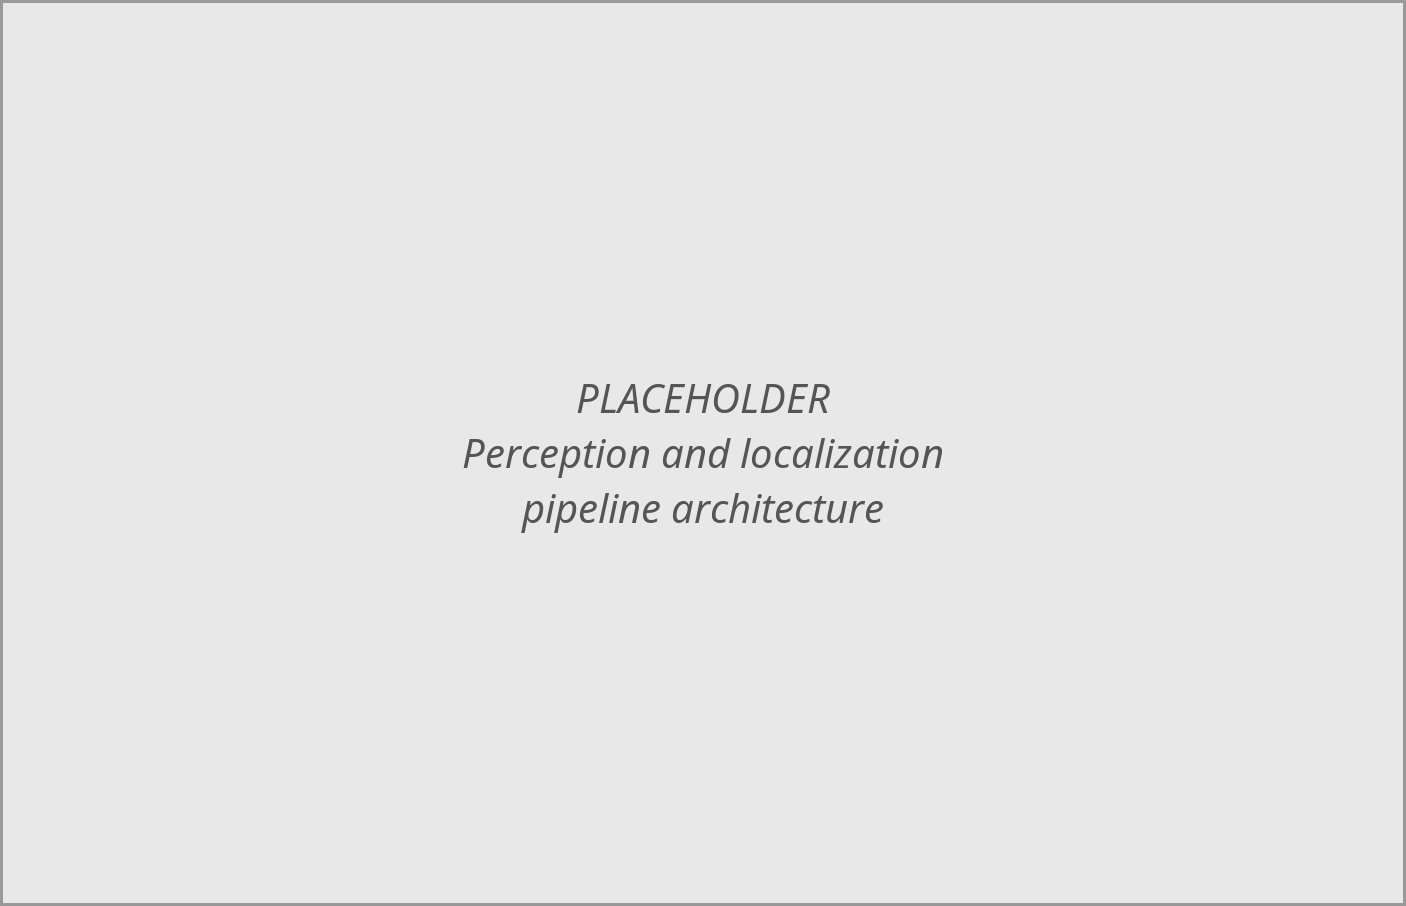
\includegraphics[width=0.85\linewidth]{teams/navigation/figures/navigational_stack}
    \caption{Perception and localization pipeline architecture}
    \label{fig:navigational_stack}
\end{figure}


\subsection{Rover Technical Budget}
\label{subsec:rover_technical_budget}

\subsubsection{Mass Budget\exampleflag}
\label{subsubsec:rover_mass_budget}
% =============================================================================
% sections/design/rover/budgets/mass.tex  -  Mass Budget
% Teams: PM / suspension (best guess - unconfirmed) / Status: stub
%
% Content required: same approach as in the Preliminary Report,
% recalculated with current, as-built figures.
% =============================================================================


\begin{table}[!t]
\centering
\caption{Rover mass budget -- mobile platform and electronics (preliminary estimate)}
\label{tab:mass_budget_mobile_arm}
\sisetup{
  group-separator      = {\,},
  group-minimum-digits = 4,
  round-mode           = places,
  round-precision      = 1
}
\setlength{\tabcolsep}{0pt}
\begin{tabular*}{\textwidth}{@{\extracolsep{\fill}}p{0.485\textwidth}@{\hspace{0.03\textwidth}}p{0.485\textwidth}@{}}
\centering
\textbf{Mobile Platform (Suspension)}\\[-2pt]
\begin{tabular}{@{}p{0.60\linewidth}c@{\hspace{8pt}}c@{}}
\toprule
\textbf{Component} & \textbf{Qty} & \textbf{Mass (kg)} \\
\midrule
Frame profiles and furniture & {---} & 5.3 \\
Body panels and box assembly & {---} & 8.1 \\[4pt]
Rocker arms & 2 & 2.0 \\
Central axis & 1 & 1.0 \\[4pt]
Hub frame and wheel disc & 4 & 6.5 \\
Tyres, TPU & 4 & 2.0 \\[4pt]
Drive motor & 4 & 5.5 \\
Wheel steering motor & 4 & 1.4 \\
\midrule
\textbf{Total (mobile platform)} & & \textbf{31.9} \\
\bottomrule
\end{tabular}
&
\centering
\textbf{Electronics and Power}\\
\begin{tabular}{@{}L{0.60\linewidth} C{0.11\linewidth} R{0.20\linewidth}@{}}
\toprule
\textbf{Component} & \textbf{Qty} & \textbf{Mass (kg)} \\
\midrule
Main compute module & 1 & 1.0 \\
Stereo camera & 1 & 0.08 \\
ToF camera & 3 & 0.15 \\
LiDAR & 1 & 0.105 \\
Battery packs & 4 & 12.0 \\
Harness, cables, and buck converters & 1 set & 1.0 \\
\midrule
\textbf{Total (electronics)} & & \textbf{13.3} \\
\bottomrule
\end{tabular}
\end{tabular*}
\end{table}

\begin{table}[!t]
\centering
\caption{Rover mass budget -- manipulator arm and science station (preliminary estimate)}
\label{tab:mass_budget_electronics_science}
\setlength{\tabcolsep}{0pt}
\begin{tabular*}{\textwidth}{@{\extracolsep{\fill}}p{0.485\textwidth}@{\hspace{0.03\textwidth}}p{0.485\textwidth}@{}}
\centering
\textbf{Manipulator Arm}\\[-2pt]
\begin{tabular}{@{}p{0.56\linewidth}c@{\hspace{8pt}}c@{}}
\toprule
\textbf{Component} & \textbf{Qty} & \textbf{Mass (kg)} \\
\midrule
Joint motors & 6 & 4.0 \\
Carbon-fiber tubes set & 1 (1 m set) & 1.9 \\
Depth camera class & 1 & 0.12 \\
Wiring and cables & 1 set & 0.5 \\
Gripper & 1 & 0.8 \\
3D-printed mounts and joint parts & 1 set & 1.5 \\
\midrule
\textbf{Total (arm subsystem)} & & \textbf{8.8} \\
\bottomrule
\end{tabular}
&
\centering
\textbf{Science Station}\\
\begin{tabular}{@{}L{0.74\linewidth} R{0.20\linewidth}@{}}
\toprule
\textbf{Component} & \textbf{Mass (kg)} \\
\midrule
Sample end-effector & 1.54 \\
Container system& 1.6 \\
Astrobio end-effector (with analyzers) & 0.7 \\
Exploration cameras & 0.16 \\
\midrule
\textbf{Total (science station)} & \textbf{4} \\
\bottomrule
\end{tabular}
\end{tabular*}
\end{table}

\begin{table}[!t]
\centering
\caption{Per-task rover configuration mass summary}
\label{tab:mass_budget_per_task_configuration}
\begin{tabular}{@{}L{2.9cm} C{1.4cm} L{3.2cm} L{4.2cm} R{2.0cm}@{}}
\toprule
\textbf{Task} & \textbf{Arm} & \textbf{Task payload/tool} & \textbf{Formula (kg)} & \textbf{Total (kg)} \\
\midrule
Navigation task    & No  & None & $35.7 + 13.3$ & 49.0 \\
Maintenance task   & Yes & None & $35.7 + 13.3 + 8.8$ & 57.8 \\
Exploration task   & No  & Exploration cameras & $35.7 + 13.3 + 0.16$ & 49.2 \\
Deep sampling task & Yes & Sample end-effector + container system & $35.7 + 13.3 + 8.8 + 1.54 + 1.6$ & 60.9 \\
Astrobiology task  & Yes & Astrobio end-effector & $35.7 + 13.3 + 8.8 + 0.7$ & 58.5 \\
Droning task       & No  & Rover-mounted landing platform & $35.7 + 13.3 + 0.8$ & 49.8 \\
\bottomrule
\end{tabular}
\end{table}

Calculation basis (
\autoref{tab:mass_budget_mobile_arm}, \autoref{tab:mass_budget_electronics_science}, \autoref{tab:mass_budget_per_task_configuration}
): base rover configuration 35.7 kg, electronics 13.3 kg, manipulator arm 8.8 kg, exploration cameras 0.16 kg, sample end-effector 1.54 kg, container system 1.6 kg, astrobio end-effector 0.7 kg, landing platform 0.8 kg (preliminary estimate).



\subsubsection{Power Budget\exampleflag}
\label{subsubsec:rover_power_budget}
% =============================================================================
% sections/design/rover/budgets/power.tex  -  Power Budget
% Teams: electronics (best guess - unconfirmed) / Status: stub
%
% Content required: amps, and other required electrical specs.
% =============================================================================


\textbf{Operating modes used in budget.}
Two modes are evaluated: \textit{Locomotion} (drive, steering, baseline electronics) and \textit{Manipulator} (arm operation with interchangeable end-effectors: gripper, auger bucket, liquid-sampling module).

\textbf{Mode 1: Locomotion (\autoref{tab:loc_power_estimate}).} Drive power is estimated from traction: \(
P_{\mathrm{loc}} = P_{\mathrm{drive}} + P_{\mathrm{steer,avg}} + P_{\mathrm{base}}.
\)

\begin{align*}
F_{\mathrm{trac}} &= mg(\sin\theta+\mu_r\cos\theta), &
T_{\mathrm{wheel}} &= \frac{F_{\mathrm{trac}}r_w}{4}, &
I_{\mathrm{drive}} &\approx 4I_{\mathrm{nom}}\frac{T_{\mathrm{wheel}}}{T_{\mathrm{nom}}}, &
P_{\mathrm{drive}} &= UI_{\mathrm{drive}}.
\end{align*}
Assumptions from \autoref{tab:motor_torque}: \(r_w=\qty{0.15}{\meter}\), \(m=\qty{75}{\kilo\gram}\), \(\theta=\ang{15}\), with motor electrical parameters \(U=\qty{48}{\volt}\), \(T_{\mathrm{nom}}=\qty{40}{\newton\meter}\), \(I_{\mathrm{nom}}=\qty{23.5}{\ampere}\).

\begin{table}[h!]
\centering
\caption{Locomotion power budget (preliminary)}
\label{tab:loc_power_estimate}
\begin{tabular}{lll}
\toprule
Term & Expression / basis & Value \\
\midrule
Drive power \(P_{\mathrm{drive}}\) &
\makecell[l]{\(\mu_r=0.10\) (compact)\\\(\mu_r=0.25\) (softer terrain)} &
\makecell[l]{\(\qty{1106}{\watt}\)\\\(\qty{1557}{\watt}\)} \\
Steering average \(P_{\mathrm{steer,avg}}\) &
\makecell[l]{\(P_{\mathrm{steer,peak}}D,\;P_{\mathrm{steer,peak}}=\qty{1636}{\watt}\)\\\(D=\numrange{0.05}{0.15}\)} &
\makecell[l]{\(\qtyrange{81.8}{245.4}{\watt}\)\\nominal \(\qty{164}{\watt}\)} \\
Baseline \(P_{\mathrm{base}}\) & conservative constant & \(\qty{96}{\watt}\) \\
Total locomotion \(P_{\mathrm{loc}}\) &
\(P_{\mathrm{drive}}+P_{\mathrm{steer,avg,nom}}+P_{\mathrm{base}}\) &
\(\qtyrange{1366}{1817}{\watt}\) \\
Locomotion energy for \(\qty{60}{\minute}\), \(E_{\mathrm{loc}}\) &
\(P_{\mathrm{loc}}\cdot \qty{1}{\hour}\) &
\(\qtyrange{1366}{1817}{\watt\hour}\) \\
\bottomrule
\end{tabular}
\end{table}

\textbf{Mode 2: Manipulator (\autoref{tab:manipulator_power_budget}).}
Manipulator-mode power is evaluated as base arm load plus end-effector increment. 
All values are preliminary (\(\pm\qty{15}{\percent}\), pending bench validation). For \numrange{3}{4} battery modules,
\[
E_{\mathrm{bat}}=\qtyrange{1728}{2304}{\watt\hour},\qquad
E_{\mathrm{loc},60}\approx\qtyrange{1366}{1817}{\watt\hour}.
\]

\begin{table}[!htbp]
\centering
\caption{Manipulator power budget (preliminary)}
\label{tab:manipulator_power_budget}
\small
\setlength{\tabcolsep}{5pt}
\renewcommand{\arraystretch}{0.95}
\begin{tabular}{p{0.34\textwidth}p{0.31\textwidth}p{0.30\textwidth}}
\toprule
Configuration / term & Expression & Power \\
\midrule
Joint actuator group \(P_{\mathrm{joint}}\) &
\(3\cdot \qty{48}{\volt}\cdot \qty{8.53}{\ampere}\) &
\(\qty{1228}{\watt}\) \\
Wrist actuator group \(P_{\mathrm{wrist}}\) &
\(3\cdot \qty{48}{\volt}\cdot \qty{2.5}{\ampere}\) &
\(\qty{360}{\watt}\) \\
Base actuator power \(P_{\mathrm{arm,motors,base}}\) &
\(P_{\mathrm{joint}}+P_{\mathrm{wrist}}\) &
\(\qty{1588}{\watt}\) \\
Auxiliary electronics \(P_{\mathrm{aux}}\) & constant & \(\qty{20}{\watt}\) \\
Base manipulator power \(P_{\mathrm{arm,base}}\) &
\(P_{\mathrm{arm,motors,base}}+P_{\mathrm{aux}}\) &
\(\qty{1608}{\watt}\) \\
\midrule
Gripper attachment &
\(\Delta P_{\mathrm{tool}}=\qtyrange{18}{36}{\watt}\) &
\(P_{\mathrm{arm,total}}=\qtyrange{1626}{1644}{\watt}\) \\
Auger bucket attachment &
\(\Delta P_{\mathrm{tool}}=\qty{35}{\watt}\) nominal (\(\qty{247}{\watt}\) short peak) &
\(P_{\mathrm{arm,total}}=\qty{1643}{\watt}\) nominal \\
Liquid-sampling attachment &
\(\Delta P_{\mathrm{liquid}}\approx\qty{20}{\watt}\) (preliminary) &
\(P_{\mathrm{arm,total}}\approx\qty{1628}{\watt}\) \\
\bottomrule
\end{tabular}
\end{table}




For the mixed \(\qty{60}{\minute}\) profile (\(t_{\mathrm{loc}}=\qty{30}{\minute}\), \(t_{\mathrm{grip}}=t_{\mathrm{auger}}=t_{\mathrm{liquid}}=\qty{10}{\minute}\)),
\[
E_{\mathrm{tot}}=
\qty{0.5}{\hour}\,P_{\mathrm{loc}}
+\qty{0.1667}{\hour}\,\bigl(P_{\mathrm{grip}}+P_{\mathrm{auger}}+P_{\mathrm{liquid}}\bigr).
\]

Using nominal values, \(E_{\mathrm{tot}}\approx\qty{1620}{\watt\hour}\). The liquid-sampling load does not change the battery-count conclusion: \num{3} modules provide limited margin, while \num{4} modules provide comfortable margin. These estimates indicate that the rover can sustain the required \(\qty{60}{\minute}\) mission duration under the considered operating profile.


\subsubsection{Data Link Budget\exampleflag}
\label{subsubsec:rover_data_link_budget}
% =============================================================================
% sections/design/rover/budgets/data_link.tex  -  Data Link Budget
% Teams: ground_station / navigation (best guess - unconfirmed) / Status: stub
%
% Content required: ground station <-> rover link budget. Open question:
% should onboard/internal communication be covered here too? Decide before
% writing.
% =============================================================================

H.265 bitrate targets are set on the Main computer using NVENC. NVENC is separate from CPU/GPU cores, 
so encoding load is low. We assume a conservative usable link capacity of 
\qty{40}{\mega\bit\per\second} (about 20\% of the \qty{200}{\mega\bit\per\second} 
802.11ac \qty{40}{\mega\hertz} peak) to account for overhead, retries, and interference.

Per-stream H.265 bitrate estimates:
\begin{itemize}
	\item Video feed: \qty{17}{\mega\bit\per\second}
	\item Telemetry + commands: $<$\qty{1}{\mega\bit\per\second}
\end{itemize}

Worst-case total is about \qty{18}{\mega\bit\per\second}, leaving about 
\qty{22}{\mega\bit\per\second} headroom (${\sim}55\%$ of estimated capacity).

\subsection{Critical Parts Required for On-Site ERC Tasks (Rover)}
\label{subsec:rover_critical_parts}

\subsubsection{Rocker-Only Suspension}
\label{subsubsec:rocker_suspension}
% =============================================================================
% sections/design/rover/critical_parts/rocker_suspension.tex  -  Rocker-Only Suspension
% Teams: suspension (best guess - unconfirmed) / Status: stub
%
% Content required:
%   - How this suspension suits us; its obstacle-overcoming capabilities
%   - Scheme with sizes
%   - Photo of suspension
%   - Photo of overcoming obstacles
% Evidence-first rule (ai_context/DECISIONS.md): lead with the
% scheme/photos, keep prose to what the figures cannot say.
% =============================================================================

\todo[inline]{How this rocker-only suspension suits us, and its
obstacle-overcoming capabilities. Maximum obstacle height, turning radiuses, maximum slope will be specified here.}

\begin{figure}[!htbp]
    \centering
    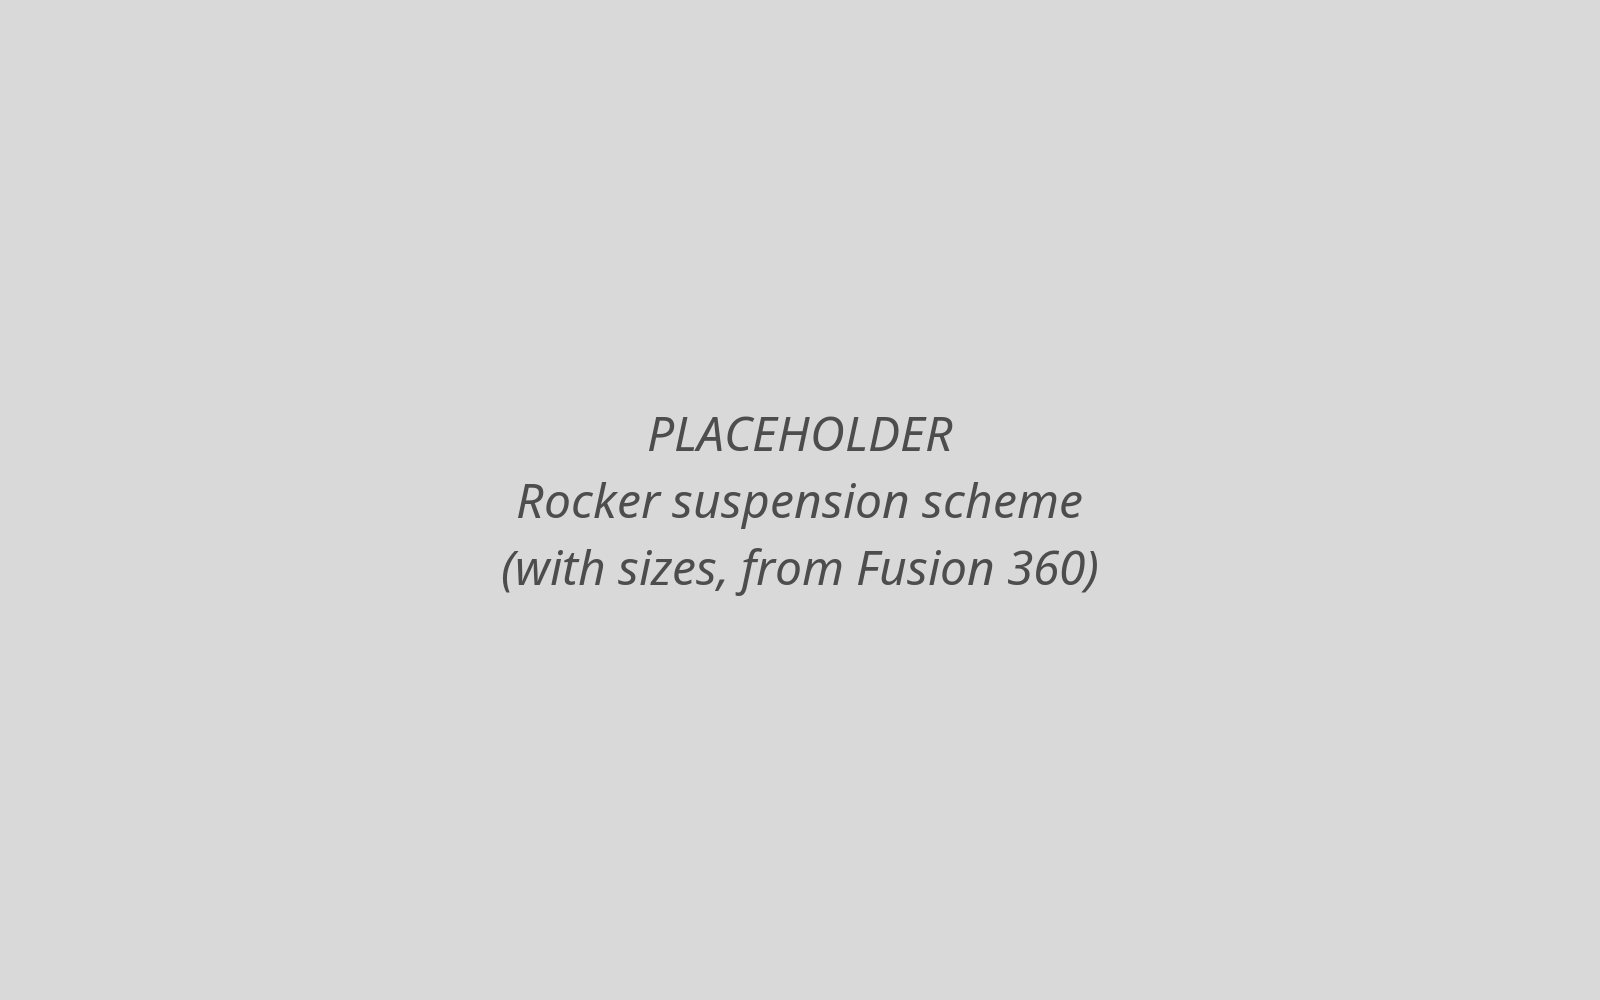
\includegraphics[width=0.8\linewidth]{teams/suspension/figures/rocker_suspension_scheme}
    \caption{Rocker suspension scheme with sizes (Fusion 360)}\label{fig:rocker_suspension_scheme}
\end{figure}

\begin{figure}[!htbp]
    \centering
    \begin{subfigure}[b]{0.48\textwidth}
        \centering
        
\includegraphics[width=\linewidth]{teams/suspension/figures/rocker_suspension_photo}
        \caption{Photo of suspension}
    \end{subfigure}
    \hfill
    \begin{subfigure}[b]{0.48\textwidth}
        \centering
        
\includegraphics[width=\linewidth]{teams/suspension/figures/rocker_suspension_obstacle}
        \caption{Photo of overcoming obstacles}
    \end{subfigure}
    \caption{Rocker suspension in operation}\label{fig:rocker_suspension_operation}
\end{figure}


\subsubsection{Wheels Design}
\label{subsubsec:wheels_design}
% =============================================================================
% sections/design/rover/critical_parts/wheels_design.tex  -  Wheels Design
% Teams: suspension / Status: in-progress
%
% Content required:
%   - Explain how this design suits us; how it benefits us on regolith
%     terrain
%   - Scheme of wheel on disc and bracket
%   - Photo during work traversing sand
% =============================================================================

\todo[inline]{Explain how this wheel design suits us, why we chose it, and how it benefits
us on regolith terrain. Physical properties of the wheels will be specified here. 
Along with sizes and weight of the wheels, and the bracket.}

\begin{figure}[!h]
    \centering
    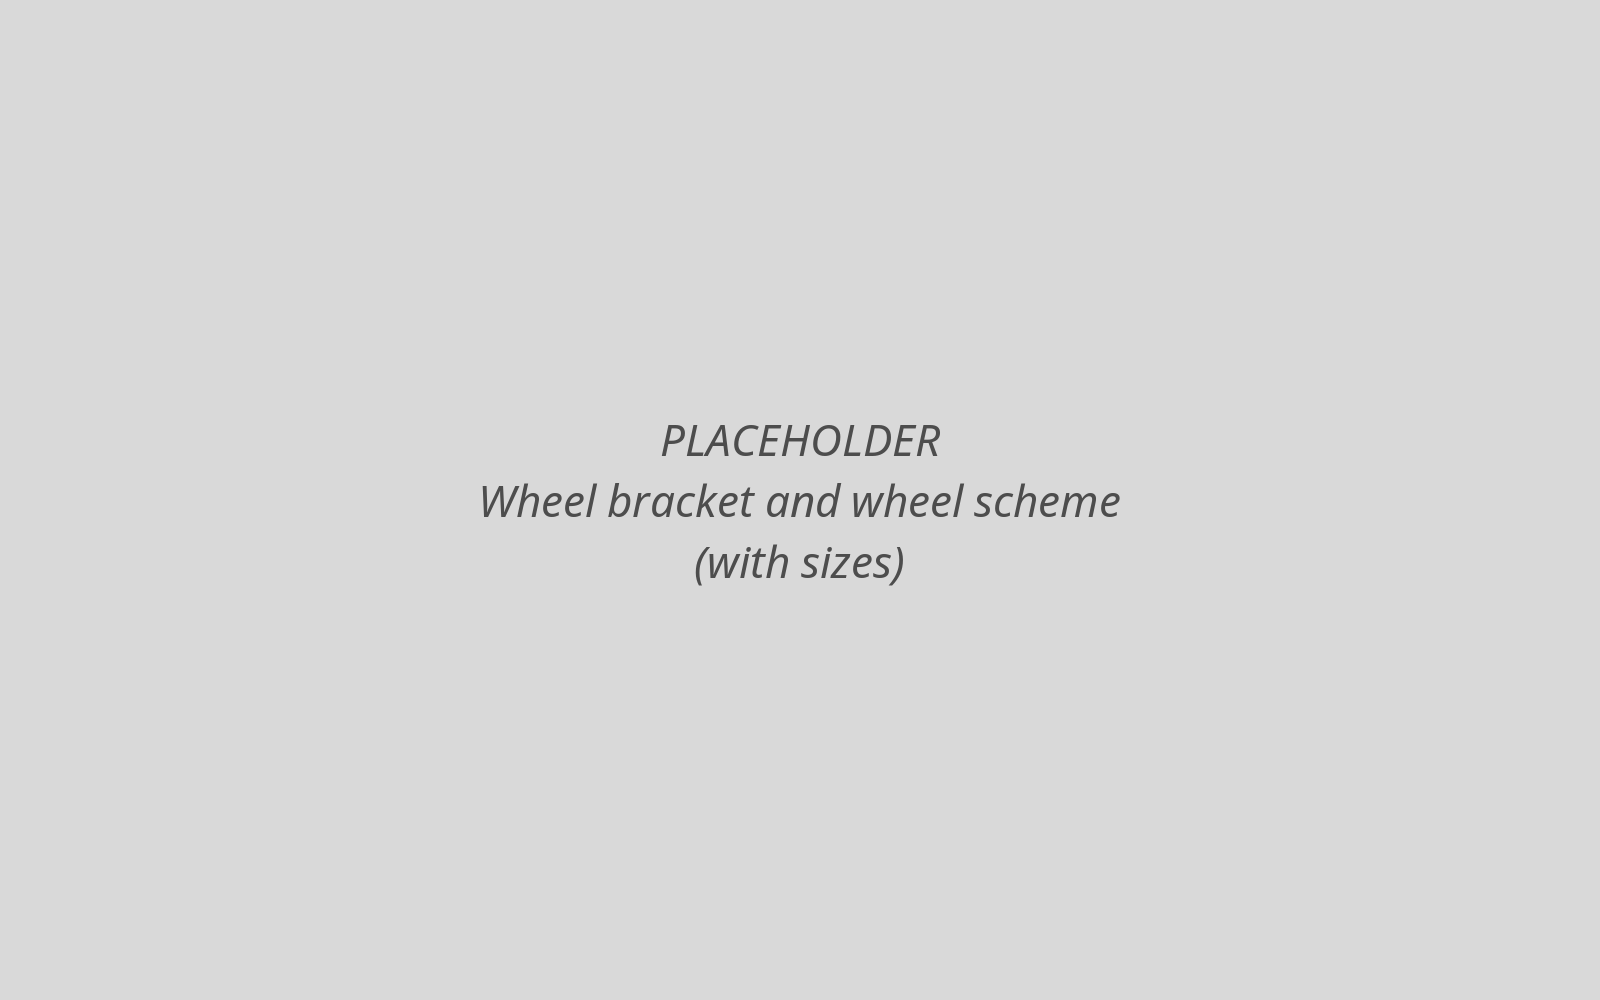
\includegraphics[width=0.8\linewidth]{teams/suspension/figures/wheel_scheme}
    \caption{Wheel and bracket scheme with sizes}\label{fig:wheel_scheme}
\end{figure}

\begin{figure}[!h]
    \centering
    
\includegraphics[width=0.6\linewidth]{teams/suspension/figures/wheel_sand_traversal}
    \caption{Wheel traversing sand}\label{fig:wheel_sand_traversal}
\end{figure}


\subsubsection{Gripper Design}
\label{subsubsec:gripper_design}
% =============================================================================
% sections/design/rover/critical_parts/gripper_design.tex - Jaw Gripper Design
% Teams: arm
% Status: draft
%
% Section title to be renamed by PM in the assembler: "Jaw Gripper Design".
%
% Images below are placeholders (teams/arm/figures/gripper_scheme.png,
% teams/arm/figures/gripper_panel_photo.png) - overwrite the same files
% with the real labeled scheme (CAD cross-section with part names: stepper
% motor, dual linkage, load sensors, rubber pads, quick-change interface)
% and a photo of the gripper working on the panel, no need to touch the
% LaTeX layout.
% =============================================================================

\todo[inline]{Write 1 short paragraph, non-obvious items only: why the
jaw gripper is a critical part — every maintenance-panel operation
(buttons, knobs, switches, card swipe, IEC~C14 plug) and probe handling
go through it; parallel-motion opening, stepper
drive with step-skipping overload protection, closed-loop force control
via two load sensors (one hardware for both delicate probes and stiff
connectors).}

The gripper mechanism and its operation on the maintenance panel are
shown in \autoref{fig:gripper_scheme_photo}.

\begin{figure}[!htbp]
    \centering
    \begin{minipage}[c]{0.40\textwidth}
        \centering
        
\includegraphics[width=\linewidth]{teams/arm/figures/gripper_scheme}
    \end{minipage}
    \hfill
    \begin{minipage}[c]{0.40\textwidth}
        \centering
        
\includegraphics[width=\linewidth]{teams/arm/figures/gripper_panel_photo}
    \end{minipage}
    \caption{Jaw gripper -- labeled scheme of the dual-linkage mechanism
    (left) and operation on the maintenance panel (right)}
    \label{fig:gripper_scheme_photo}
\end{figure}

\subsubsection{Astro-Bio Gripper}
\label{subsubsec:astrobio_gripper}
% =============================================================================
% sections/design/rover/critical_parts/astrobio_gripper.tex  -  Astro-Bio Gripper
% Teams: arm (best guess - unconfirmed) / Status: stub
%
% Content required: same format as gripper_design.tex (characteristics,
% size, capabilities; detailed scheme with named parts; photo of working
% on panel).
% Evidence-first rule (ai_context/DECISIONS.md): lead with the
% scheme/photo, keep prose to what the figures cannot say.
%
% NOTE: possible overlap with rover/robotic_arm_6dof.tex - coordinate
% to avoid duplicate content.
% =============================================================================

\todo[inline]{Astro-bio gripper. Same format as Gripper Design.}


\subsubsection{6-DOF Manipulator}
\label{subsubsec:manipulator_6dof}
% =============================================================================
% sections/design/rover/critical_parts/manipulator_6dof.tex  -  6-DOF Manipulator
% Teams: arm (owner: Martha) / Status: stub
%
% Content required: not yet defined. Decomposition and content owned by
% Martha. If this splits into multiple leaf files, update the assembler
% (sections/03_final_design_description.tex) accordingly rather than
% cramming everything into this one file.
% =============================================================================

\todo[inline]{6-DOF manipulator. Decomposition and content owned by
Martha.}


\subsection{Rover Innovative Design Solutions}
\label{subsec:rover_innovations}

\subsubsection{Unified Sample Gripper}
\label{subsubsec:unified_sample_gripper}
% =============================================================================
% sections/design/rover/innovations/unified_sample_gripper.tex  -  Unified Sample Gripper
% Teams: arm (best guess - unconfirmed) / Status: stub
%
% Content required: not yet defined. No figure/content requirements have
% been sketched yet.
% =============================================================================

\todo[inline]{Unified sample gripper. Content requirements not yet
defined.}


\subsection{Drone Design Description}
\label{subsec:drone_design_description}

\todo[inline]{Drone design description. Not yet discussed by the team.
Decompose into leaf files under sections/design/drone/ analogous to the
Rover Design Description above once defined. Jury feedback (Preliminary):
the drone was never actually shown despite an extensive description - lead
with real photos.}

\subsection{Drone Technical Budget}
\label{subsec:drone_technical_budget}

\todo[inline]{Drone technical budget: mass, power, data link. Not yet
discussed - the Preliminary Report's drone budget was missing a data link
figure entirely; the rubric scores mass + power + data link together.}

\subsection{Critical Parts Required for On-Site ERC Tasks (Drone)}
\label{subsec:drone_critical_parts}

\todo[inline]{Drone critical parts for on-site ERC tasks. Not yet
discussed.}

\subsection{Drone Innovative Design Solutions}
\label{subsec:drone_innovations}

\todo[inline]{Drone innovative design solutions. Not yet discussed. Note:
this subsection scores 0 pts if the drone is fully COTS.}
